% -*- coding: UTF-8 -*-
% hurlex-chapt6.tex
% hurlex 开发文档 第6章内容

\section {添加全局段描述符表}

\subsection{保护模式的引入}

\par 从本章开始,我们就要开始涉及到x86保护模式编程的一些细节问题了。

\par 我们从80386处理器入手。首先,到了80386时代,CPU有了四种运行模式,即实模式、保护模式、虚拟8086模式和SMM模式。

\par 模式指的是8086CPU的运行模式,不过这是后来提出的概念,在8086时代只有当时的运行模式,自然也就没有"实模式"这么个提法。\allowbreak
如果世界上只有一种性别的人,也就没有男人,女人这种名称了。8086的汇编中,我们对于实模式的各种机制应该算是比较了解了,其\allowbreak
大致包括实模式1MB的线性地址空间、内存寻址方法、寄存器、端口读写以及中断处理方法等内容。

\par 不过到了80386时代,引进了一种沿用至今的CPU运行机制——保护模式(Protected Mode)。保护模式有一些新的特色,用来增强多工\allowbreak
和系统稳定度,比如内存保护,分页系统,以及硬件支持的虚拟内存等。大部分现今基于x86架构的操作系统都在保护模式下运行,\allowbreak
包括Linux、FreeBSD、以及微软Windows 2.0和之后版本(都指32位操作系统) 。

\par 虚拟8086模式用于在保护模式下运行原来实模式下的16位程序,我们不关心。SMM模式是不对程序员开放的,所以我们也不关心。

\par 我们先来研究保护模式,在保护模式里80386首先扩展了8086的处理器\footnote{其实中间有个80286,不过这是个过渡产品。},\allowbreak
原先的AX,BX,CX,DX,SI,DI,SP,BP从16位扩展(Extend)到了32位,并改名EAX,EBX,ECX,EDX,ESI,EDI,ESP,EBP,E\allowbreak
就是Extend的意思。当然,保留了原先的16位寄存器的使用习惯,就像在8086下能用AH和AL访问AX的高低部分一样,不过EAX的低\allowbreak
位部分能使用AX直接访问,高位却没有直接的方法,只能通过数据右移16位之后再访问。另外,CS,DS,ES,SS这几个16位段寄存器\allowbreak
保留,再增加FS,GS两个段寄存器。另外还有其它很多新增加的寄存器。本着实用原则,到时候用到了我们再说。

\subsection{保护模式下的内存分段}

\par 我们知道,对CPU来讲,系统中的所有储存器中的储存单元都处于一个统一的逻辑储存器中,它的容量受CPU寻址能力的限制。\allowbreak
这个逻辑储存器就是我们所说的线性地址空间。8086有20位地址线,拥有1MB的线性地址空间。而80386有32位地址线,拥有4GB的\allowbreak
线性地址空间。但是80386依旧保留了8086采用的地址分段的方式,只是增加了一个折中的方案,即只分一个段,段基址0×00000000,\allowbreak
段长0xFFFFFFFF(4GB),这样的话整个线性空间可以看作就一个段,这就是所谓的平坦模型(Flat Mode)。

\par  我们先来看保护模式下的内存是如何分段管理的。为了便于理解,我们从一个设计者的角度来研究这个问题,顺便试图按我的理\allowbreak
解对一些机制的设计原因做一些阐释。

\par 首先是对内存分段中每一个段的描述,实模式对于内存段并没有访问控制,任意的程序可以修改任意地址的变量,而保护模式需要\allowbreak
对内存段的性质和允许的操作给出定义,以实现对特定内存段的访问检测和数据保护。考虑到各种属性和需要设置的操作,32位保护模式\allowbreak
下对一个内存段的描述需要8个字节,其称之为段描述符(Segment Descriptor)。段描述符分为数据段描述符、指令段描述符\allowbreak
和系统段描述符三种。

\par 我们现在看一张段描述符的8个字节的分解图吧,至于每一个细节的含义请大家自行查阅Intel文档。\allowbreak
\footnote{本章很多图片直接引用自《Intel® 64 and IA-32 Architectures Software Developer’s Manual Vol-ume3 :
System Programming Guide》,下文不再声明。}

\begin{figure}[ht]
      \centering
      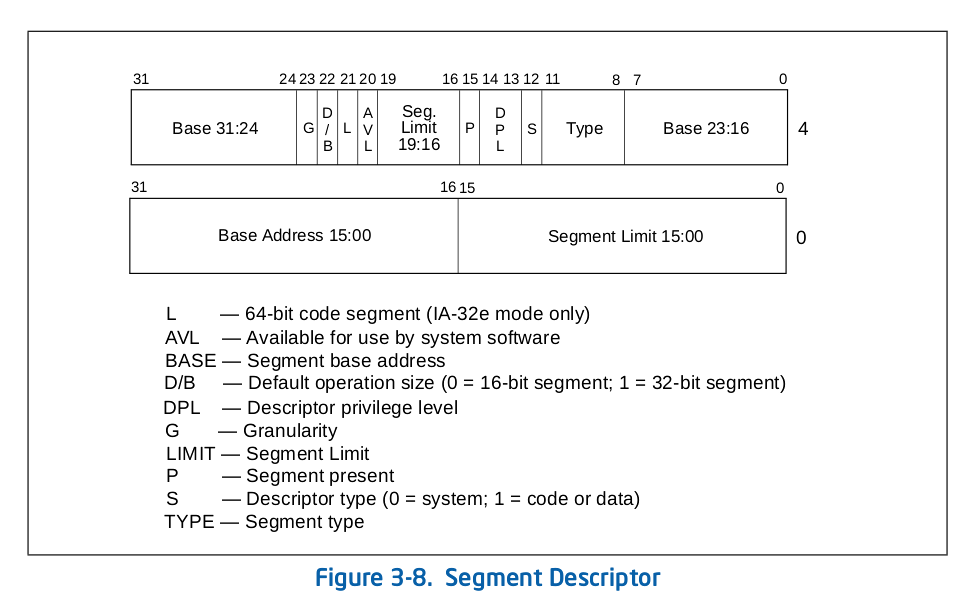
\includegraphics[scale=0.45]{picture/chapt6/segment_descriptor.png}
      \caption{段描述符的结构}
\end{figure}

 \par 显然,寄存器不足以存放N多个内存段的描述符集合,所以这些描述符的集合(称之为描述符表)被放置在内存里了。\allowbreak
 在很多描述符表中,最重要的就是所谓的全局描述符表(Global Descriptor Table,GDT),它为整个软硬件系统服务。

 \par 一个问题解决了,但是又引出了的其他问题。问题一:这些描述符表放置在内存哪里?答案是没有固定的位置,可以任由\allowbreak
 程序员安排在任意合适的位置。问题一带出了问题二:既然没有指定固定位置,CPU如何知道全局描述符表在哪?答案是Intel干脆设置了\allowbreak
 一个48位的专用的全局描述符表寄存器(GDTR)来保存全局描述符表的信息。那这48位怎么分配呢?如图所示,0-15位表示GDT\allowbreak
 的边界位置(数值为表的长度-1,因为从0计算),16-47位这32位存放的就是GDT的基地址(恰似数组的首地址)。

\begin{figure}[ht]
      \centering
      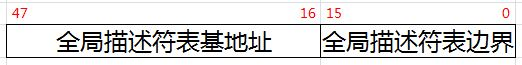
\includegraphics[scale=0.5]{picture/chapt6/gdtr.png}
      \caption{GDTR的结构}
\end{figure}

\par 既然用16位来表示表的长度,那么2的16次方就是65536字节,除以每一个描述符的8字节,那么最多能创建8192个描述符。

\par 貌似说了这么多,我们一直还没提CPU的默认工作方式。80386CPU加电的时候自动进入实模式\footnote{实际上此时CPU还不是\allowbreak
彻底的实模式,之后第二条指令才进入彻底的实模式。对这个问题的讨论超出本文档的范围,所以不再讨论。}既然CPU加电后就一直\allowbreak
工作在实模式下了。那怎么进入保护模式呢?说来也简单,80386CPU内部有5个32位的控制寄存器(Control Register,CR),\allowbreak
分别是CR0到CR3,以及CR8。用来表示CPU的一些状态,其中的CR0寄存器的PE位(Protection Enable,保护模式允许位),0号位,\allowbreak
就表示了CPU的运行状态,0为实模式,1为保护模式。通过修改这个位就可以立即改变CPU的工作模式。

\begin{figure}[ht]
      \centering
      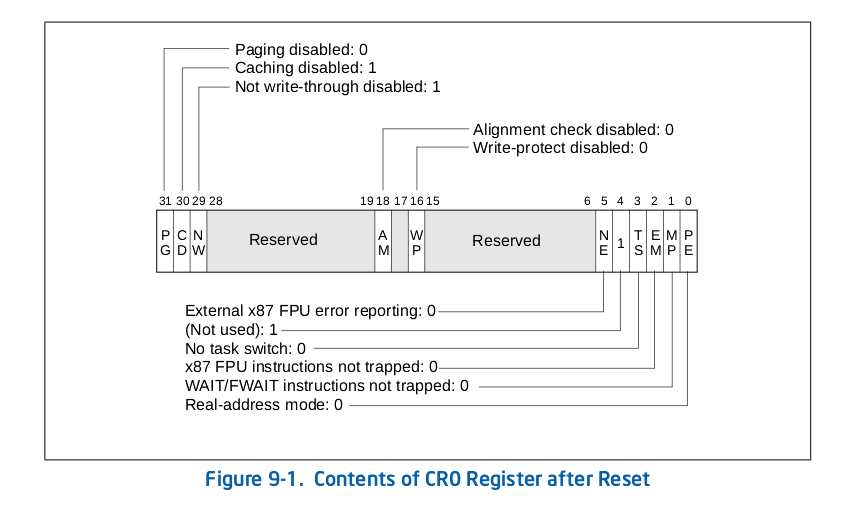
\includegraphics[scale=0.5]{picture/chapt6/cr0.png}
      \caption{CR0寄存器的结构}
\end{figure}

\par 不过需要注意的是,一旦CR0寄存器的PE位被修改,CPU就立即按照保护模式去寻址了,所以这就要求我们必须在进入保护模式\allowbreak
之前就在内存里放置好GDT,然后设置好GDTR寄存器。我们知道实模式下只有1MB的寻址空间,所以GDT就等于被限制在了这里。即便\allowbreak
是再不乐意我们也没有办法,只得委屈就全的先安排在这里。不过进入保护模式之后我们就可以在4G的空间里设置并修改原来的GDTR了。

\par OK,现在有了描述符的数组了,也有了“数组指针”(GDTR)了,怎么表示我们要访问哪个段呢?还记得8086时代的段寄存器吧?\allowbreak
不过此时它们改名字了,叫段选择器(段选择子)。此时的CS等寄存器不再保存段基址了,而是保存其指向段的索引信息,CPU会根据\allowbreak
这些信息在内存中获取到段信息。

\par 地址合成的过程如下图所示:

\begin{figure}[ht]
      \centering
      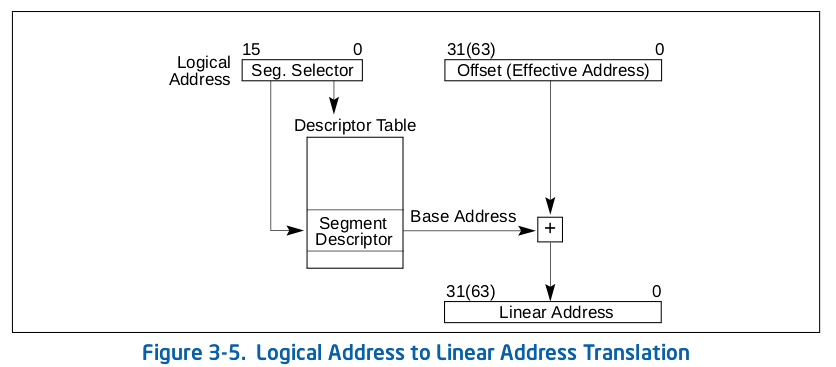
\includegraphics[scale=0.5]{picture/chapt6/protected_segment_addr.png}
      \caption{段机制的地址合成过程}
\end{figure}

\par 以上就是对x86保护模式的阐述了,细节问题希望大家能结合之后的代码自行参考Intel文档学习。

\subsection{具体采用的分段策略}

\par 下面开始针对我们的内核给出具体的设计方案了。我们之前简单的阐述了分段,事实上现代操作系统几乎不再使用分段而是绕过\allowbreak
分段技术直接使用了分页。其实分段和分页没什么必然联系。只不过Intel从8086开始,其制造的CPU就以段地址+偏移地址的方式来访问内存。\allowbreak
后来要兼容以前的CPU,Intel不得不一直保留着这个传统。分段可以说是Intel的CPU一直保持着的一种机制,而分页只是保护模式下\allowbreak
的一种内存管理策略。不过想开启分页机制,CPU就必须工作在保护模式,而工作在保护模式时候可以不开启分页。所以事实上分段是\allowbreak
必须的,而分页是可选的。

\par 那我们如何"绕过"这个分段机制呢?不知道大家是否还记得之前我们所说的平坦模式(Flat Mode)?这就是我们"绕过"的\allowbreak
方法。当整个虚拟地址空间是一个起始地址为0,限长为4G的"段"时,我们给出的偏移地址就在数值上等于是段机制处理之后的地址了。
不过我们不是简单的对所有的段使用同样的描述符,而是给代码段和数据段分配不同的描述符。下面的示意图描述了这个抽象:

\begin{figure}[ht]
      \centering
      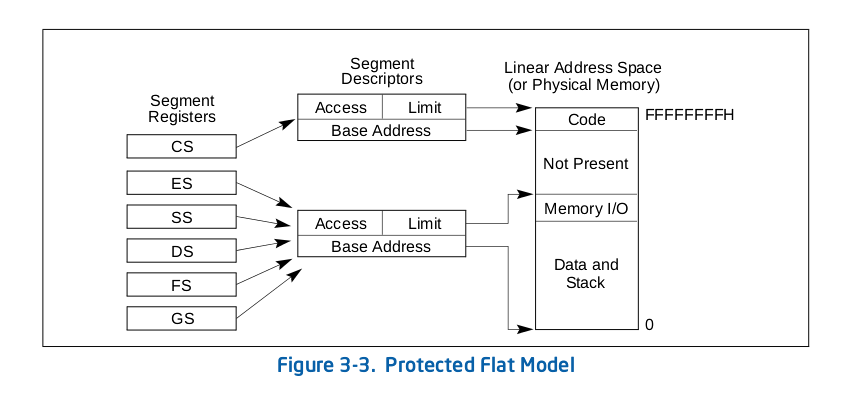
\includegraphics[scale=0.5]{picture/chapt6/protected_flat_mode.png}
      \caption{带有保护的平坦模式}
\end{figure}

\par 在第二章中我们谈到了GRUB在载入内核时候的一些状态,其中就有以下两条:

\begin{mdframed}
	\begin{enumerate}
		\item CS 指向基地址为 0x00000000,限长为4G – 1的代码段描述符。
		\item DS,SS,ES,FS 和 GS 指向基地址为0x00000000,限长为4G–1的数据段描述符。
	\end{enumerate}
\end{mdframed}

\par 大家现在应该理解这两项了吧?既然GRUB已经替我们做过了,那我们还有必要再来一次吗?当然有必要了,一来是学习的必要,\allowbreak
二来在后期实现TSS任务切换的时候还要用到全局描述符表。

\par 下面我们给出具体的实现代码,首先是头文件和一些定义:

\begin{lstlisting}[language = C, caption = include/gdt.h]
#ifndef INCLUDE_GDT_H_
#define INCLUDE_GDT_H_

#include "types.h"

// 全局描述符类型
typedef
struct gdt_entry_t {
	uint16_t limit_low;     // 段界限   15 ~ 0
	uint16_t base_low;      // 段基地址 15 ~ 0
	uint8_t  base_middle;   // 段基地址 23 ~ 16
	uint8_t  access;        // 段存在位、描述符特权级、描述符类型、描述符子类别
	uint8_t  granularity; 	// 其他标志、段界限 19 ~ 16
	uint8_t  base_high;     // 段基地址 31 ~ 24
} __attribute__((packed)) gdt_entry_t;

// GDTR
typedef
struct gdt_ptr_t {
	uint16_t limit; 	// 全局描述符表限长
	uint32_t base; 		// 全局描述符表 32 位基地址
} __attribute__((packed)) gdt_ptr_t;

// 初始化全局描述符表
void init_gdt();

// GDT 加载到 GDTR 的函数[汇编实现]
extern void gdt_flush(uint32_t);

#endif 	// INCLUDE_GDT_H_
\end{lstlisting}

\par 结合上面关于全局段描述符表的格式说明,这两个结构体的定义应该很容易看懂。具体的函数实现如下:

\begin{lstlisting}[language = C, caption = gdt/gdt.c]
#include "gdt.h"
#include "string.h"

// 全局描述符表长度
#define GDT_LENGTH 5

// 全局描述符表定义
gdt_entry_t gdt_entries[GDT_LENGTH];

// GDTR
gdt_ptr_t gdt_ptr;

static void gdt_set_gate(int32_t num, uint32_t base,
			uint32_t limit, uint8_t access, uint8_t gran);

// 声明内核栈地址
extern uint32_t stack;

// 初始化全局描述符表
void init_gdt()
{
	// 全局描述符表界限 e.g. 从 0 开始,所以总长要 - 1
	gdt_ptr.limit = sizeof(gdt_entry_t) * GDT_LENGTH - 1;
	gdt_ptr.base = (uint32_t)&gdt_entries;

	// 采用 Intel 平坦模型
	gdt_set_gate(0, 0, 0, 0, 0);   // 按照 Intel 文档要求,第一个描述符必须全 0
	gdt_set_gate(1, 0, 0xFFFFFFFF, 0x9A, 0xCF); 	// 指令段
	gdt_set_gate(2, 0, 0xFFFFFFFF, 0x92, 0xCF); 	// 数据段
	gdt_set_gate(3, 0, 0xFFFFFFFF, 0xFA, 0xCF); 	// 用户模式代码段
	gdt_set_gate(4, 0, 0xFFFFFFFF, 0xF2, 0xCF); 	// 用户模式数据段

	// 加载全局描述符表地址到 GPTR 寄存器
	gdt_flush((uint32_t)&gdt_ptr);
}

// 全局描述符表构造函数,根据下标构造
// 参数分别是 数组下标、基地址、限长、访问标志,其它访问标志
static void gdt_set_gate(int32_t num, uint32_t base, uint32_t limit, uint8_t access, uint8_t gran)
{
	gdt_entries[num].base_low     = (base & 0xFFFF);
	gdt_entries[num].base_middle  = (base >> 16) & 0xFF;
	gdt_entries[num].base_high    = (base >> 24) & 0xFF;

	gdt_entries[num].limit_low    = (limit & 0xFFFF);
	gdt_entries[num].granularity  = (limit >> 16) & 0x0F;

	gdt_entries[num].granularity |= gran & 0xF0;
	gdt_entries[num].access       = access;
}

\end{lstlisting}

\par 这里唯一麻烦的就是需要对照着Intel文档的说明,去为每一个段描述符计算权限位的数值了。\allowbreak
至于加载全局描述符表的操作,为了方便期间我们直接用汇编语言实现了,代码如下:\allowbreak
\footnote{这里需要强调的是这里的代码文件命名为gdt\_s.s,因为同一个目录下的.s和.c文件都会被编译为同名的.o文件,所以同名的话\allowbreak
会被相互覆盖掉。}

\begin{lstlisting}[language = {[x86masm]Assembler}, caption = gdt/gdt\_s.s]
[GLOBAL gdt_flush]

gdt_flush:
	mov eax, [esp+4]  ; 参数存入 eax 寄存器
	lgdt [eax]        ; 加载到 GDTR [修改原先GRUB设置]

	mov ax, 0x10      ; 加载我们的数据段描述符
	mov ds, ax        ; 更新所有可以更新的段寄存器
	mov es, ax
	mov fs, ax
	mov gs, ax
	mov ss, ax
	jmp 0x08:.flush   ; 远跳转, 0x08 是我们的代码段描述符
			  ; 远跳目的是清空流水线并串行化处理器
.flush:
	ret
\end{lstlisting}

\par 我想这个汇编函数中唯一需要解释的就是jmp跳转那一句了,首先0×08是我们跳转目标段的段选择子(这个不陌生吧?),\allowbreak
其对应段描述符第2项。后面的跳转目标标号可能会让你诧异,因为它就是下一行代码。这是为何?当然有深意了,第一,Intel不\allowbreak
允许直接修改段寄存器cs的值,我们只好这样通过这种方式更新cs段寄存器;第二,x86以后CPU所增加的指令流水线和高速缓存可能\allowbreak
会在新的全局描述符表加载之后依旧保持之前的缓存,那么修改GDTR之后最安全的做法就是立即清空流水线和更新高速缓存。说的这么\allowbreak
牛逼的样子,其实只要一句jmp跳转就能强迫CPU自动更新了,很简单吧?

\par 到这里段描述符表的创建就告一段落了,其实我们完全可以直接计算出这些段具体的表示数值然后硬编码进去,但是出于学习的\allowbreak
目的,我们还是写了这些函数进行处理。当然了,我们没有谈及一些具体的描述符细节问题,因为Intel文档的描述都很详细。

\par 创建好所有的文件以后,再次修改入口函数如下:

\begin{lstlisting}[language = C, caption = init/entry.c]
#include "gdt.h"
#include "console.h"
#include "debug.h"

int kern_entry()
{
	init_debug();
	init_gdt();

	console_clear();
	printk_color(rc_black, rc_green, "Hello, OS kernel!\n");

	return 0;
}
\end{lstlisting}

\par 编译运行后如果输出了正常的信息,就说明我们成功了。于是,本章结束。
